
\documentclass[varwidth,border=20pt]{standalone}
\usepackage{tikz}
\usetikzlibrary{arrows.meta}
\usetikzlibrary{shapes}
\usetikzlibrary{backgrounds,shadows}

\begin{document}  
\begin{figure}
    \centering
    %Process: PROCESS1
    \begin{tikzpicture}[baseline, y=-0.7cm]
    
        % Declare the states
        \node[draw, ellipse] at (0, 0) (00) {$0$};
        \node[draw, ellipse] at (6, 0) (10) {$1$};
        \node[draw, ellipse] at (3, 0) (A0) {$A_0$};
        \node[draw, ellipse] at (3, 3) (A1) {$A_1$};
        \node[draw, ellipse] at (3, 6) (A2) {$A_2$};
        \node[draw, ellipse] at (3, 9) (A3) {$A_3$};
        \node[draw, ellipse] at (3, 12) (A4) {$A_4$};
    
        % Declare edges
        \draw[->] (A0) -- (00) node[midway,below] {a};
        \draw[->] (A0) -- (A1) node[midway,left] {a};
        \draw[->] (A1) -- (A2) node[midway,left] {a};
        \draw[->] (A2) -- (A3) node[midway,left] {a};
        \draw[->] (A3) -- (A4) node[midway,left] {a};
        \draw[->] (A4) -- (10) node[midway,above,right] {a};
    
        % Declare initial edges
        \draw[->] (2, -1) -- (A0) node[midway] {};
    
        % Declare final edges
        \draw[->] (10) -- (7, -1) node[midway] {};
        \draw[->] (A0) -- (4, -1) node[midway] {};
    
    \end{tikzpicture}
    \caption{We do it once.}
    \label{fig:process1}
\end{figure}
\vspace{2em}
 
\begin{figure}
    \centering
    %Process: PROCESS2
    \begin{tikzpicture}[baseline, y=-0.7cm]
    
        % Declare the states
        \node[draw, ellipse] at (0, 0) (00) {$0$};
        \node[draw, ellipse] at (6, 0) (10) {$1$};
        \node[draw, ellipse] at (3, 0) (A0) {$A_0$};
        \node[draw, ellipse] at (3, 3) (A1) {$A_1$};
        \node[draw, ellipse] at (3, 6) (A2) {$A_2$};
        \node[draw, ellipse] at (3, 9) (A3) {$A_3$};
        \node[draw, ellipse] at (3, 12) (A4) {$A_4$};
    
        % Declare edges
        \draw[->] (A0) -- (00) node[midway,below] {a};
        \draw[->] (A0) -- (A1) node[midway,left] {a};
        \draw[->] (A1) -- (A2) node[midway,left] {a};
        \draw[->] (A2) -- (A3) node[midway,left] {a};
        \draw[->] (A3) -- (A4) node[midway,left] {a};
        \draw[->] (A4) -- (10) node[midway,above,right] {a};
    
        % Declare initial edges
        \draw[->] (2, -1) -- (A0) node[midway] {};
    
        % Declare final edges
        \draw[->] (10) -- (7, -1) node[midway] {};
        \draw[->] (A0) -- (4, -1) node[midway] {};
    
    \end{tikzpicture}
    \caption{We do it twice.}
    \label{fig:process2}
\end{figure}
\vspace{2em}
 
\begin{figure}
    \centering
    %Process: PROCESS3
    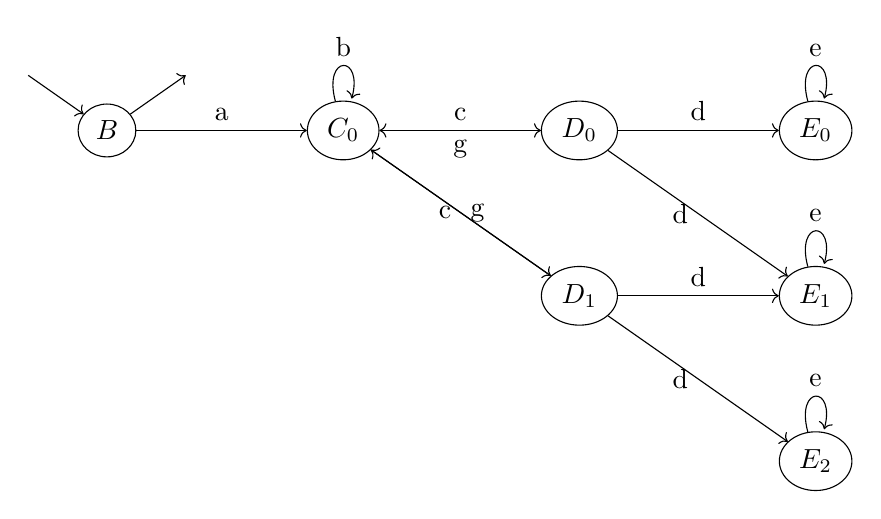
\begin{tikzpicture}[baseline, y=-0.7cm]
    
        % Declare the states
        \node[draw, ellipse] at (0, 0) (B0) {$B$};
        \node[draw, ellipse] at (3, 0) (C0) {$C_0$};
        \node[draw, ellipse] at (6, 0) (D0) {$D_0$};
        \node[draw, ellipse] at (6, 3) (D1) {$D_1$};
        \node[draw, ellipse] at (9, 0) (E0) {$E_0$};
        \node[draw, ellipse] at (9, 3) (E1) {$E_1$};
        \node[draw, ellipse] at (9, 6) (E2) {$E_2$};
    
        % Declare edges
        \draw[->] (B0) -- (C0) node[midway,above] {a};
        \draw[->] (C0) edge[loop above] node[midway, above] {b} (C0);
        \draw[->] (C0) -- (D0) node[midway,above] {c};
        \draw[->] (C0) -- (D1) node[midway,above,left] {c};
        \draw[->] (D0) -- (C0) node[midway,below] {g};
        \draw[->] (D0) -- (E0) node[midway,above] {d};
        \draw[->] (D0) -- (E1) node[midway,above,left] {d};
        \draw[->] (D1) -- (C0) node[midway,below,right] {g};
        \draw[->] (D1) -- (E1) node[midway,above] {d};
        \draw[->] (D1) -- (E2) node[midway,above,left] {d};
        \draw[->] (E0) edge[loop above] node[midway, above] {e} (E0);
        \draw[->] (E1) edge[loop above] node[midway, above] {e} (E1);
        \draw[->] (E2) edge[loop above] node[midway, above] {e} (E2);
    
        % Declare initial edges
        \draw[->] (-1, -1) -- (B0) node[midway] {};
    
        % Declare final edges
        \draw[->] (B0) -- (1, -1) node[midway] {};
    
    \end{tikzpicture}
    \caption{More complex this time.}
    \label{fig:process3}
\end{figure}
\vspace{2em}
 
%Process: PROCESS4
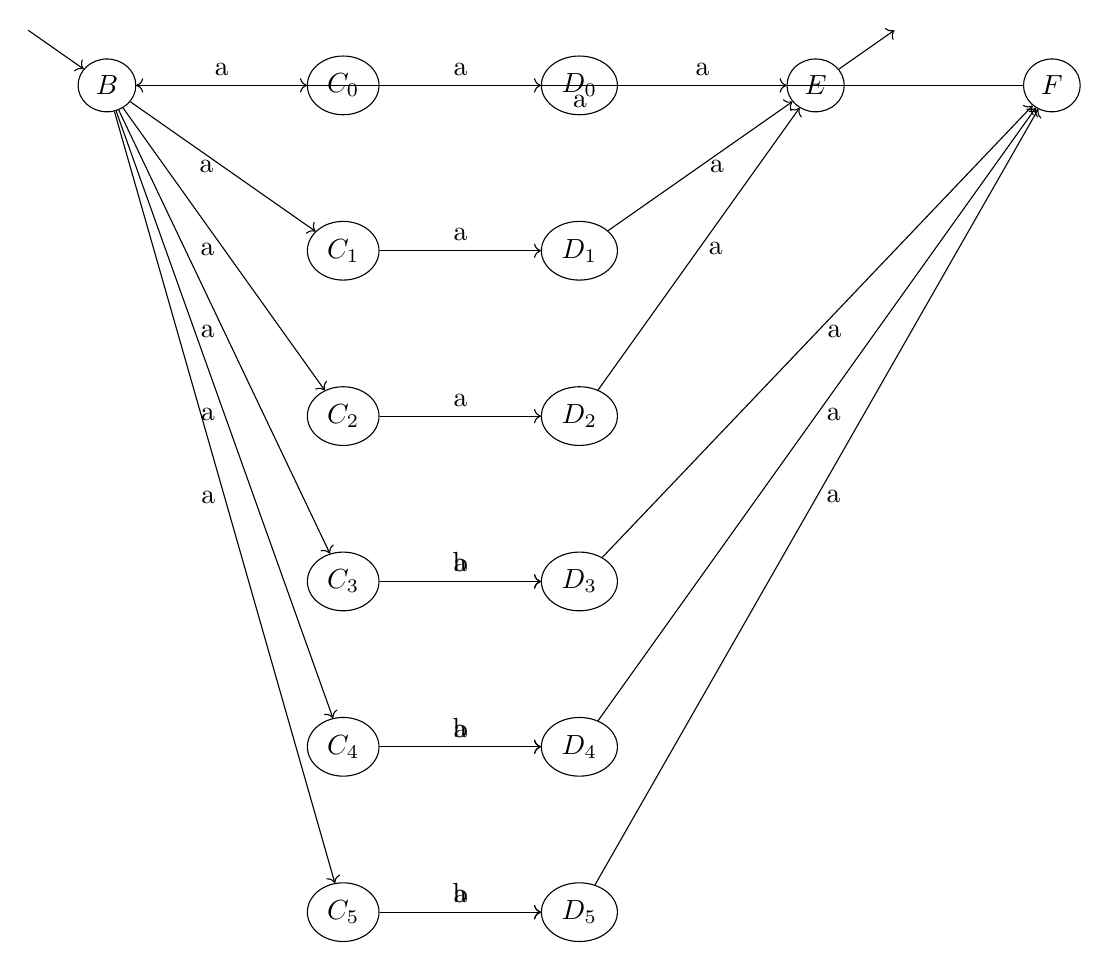
\begin{tikzpicture}[baseline, y=-0.7cm]

    % Declare the states
    \node[draw, ellipse] at (0, 0) (B0) {$B$};
    \node[draw, ellipse] at (3, 0) (C0) {$C_0$};
    \node[draw, ellipse] at (3, 3) (C1) {$C_1$};
    \node[draw, ellipse] at (3, 6) (C2) {$C_2$};
    \node[draw, ellipse] at (3, 9) (C3) {$C_3$};
    \node[draw, ellipse] at (3, 12) (C4) {$C_4$};
    \node[draw, ellipse] at (3, 15) (C5) {$C_5$};
    \node[draw, ellipse] at (6, 0) (D0) {$D_0$};
    \node[draw, ellipse] at (6, 3) (D1) {$D_1$};
    \node[draw, ellipse] at (6, 6) (D2) {$D_2$};
    \node[draw, ellipse] at (6, 9) (D3) {$D_3$};
    \node[draw, ellipse] at (6, 12) (D4) {$D_4$};
    \node[draw, ellipse] at (6, 15) (D5) {$D_5$};
    \node[draw, ellipse] at (9, 0) (E0) {$E$};
    \node[draw, ellipse] at (12, 0) (F0) {$F$};

    % Declare edges
    \draw[->] (B0) -- (C0) node[midway,above] {a};
    \draw[->] (B0) -- (C1) node[midway,above,left] {a};
    \draw[->] (B0) -- (C2) node[midway,above,left] {a};
    \draw[->] (B0) -- (C3) node[midway,above,left] {a};
    \draw[->] (B0) -- (C4) node[midway,above,left] {a};
    \draw[->] (B0) -- (C5) node[midway,above,left] {a};
    \draw[->] (C0) -- (D0) node[midway,above] {a};
    \draw[->] (C1) -- (D1) node[midway,above] {a};
    \draw[->] (C2) -- (D2) node[midway,above] {a};
    \draw[->] (C3) -- (D3) node[midway,above] {a};
    \draw[->] (C3) -- (D3) node[midway,above] {b};
    \draw[->] (C4) -- (D4) node[midway,above] {a};
    \draw[->] (C4) -- (D4) node[midway,above] {b};
    \draw[->] (C5) -- (D5) node[midway,above] {a};
    \draw[->] (C5) -- (D5) node[midway,above] {b};
    \draw[->] (D0) -- (E0) node[midway,above] {a};
    \draw[->] (D1) -- (E0) node[midway,above,right] {a};
    \draw[->] (D2) -- (E0) node[midway,above,right] {a};
    \draw[->] (D3) -- (F0) node[midway,above,right] {a};
    \draw[->] (D4) -- (F0) node[midway,above,right] {a};
    \draw[->] (D5) -- (F0) node[midway,above,right] {a};
    \draw[->] (F0) -- (B0) node[midway,below] {a};

    % Declare initial edges
    \draw[->] (-1, -1) -- (B0) node[midway] {};

    % Declare final edges
    \draw[->] (E0) -- (10, -1) node[midway] {};

\end{tikzpicture}
\vspace{2em}
\end{document}